\documentclass[11pt,a4paper]{article}
\usepackage[utf8]{inputenc}
\usepackage{amsmath}
\usepackage{amsfonts}
\usepackage{amssymb}
\usepackage{graphicx}
\graphicspath{ {./images/} }
\author{Bianca}
\DeclareMathOperator*{\argmin}{argmin}
\DeclareMathOperator*{\diag}{diag}
\begin{document}
\begin{flushleft}
\section{Linear Models}
\subsection{Overfitting}
\begin{itemize}
\item fitting: der Prozess die Parameter einer Modelfunktion y so anzupassen das sie der der Beispieldaten D am besten passen
\item overfiiting: "Fitting the data more than is warranted"
\item alias besser passen als berechtigt?
\item Gründe:
	\begin{itemize}
	\item zu komplizierte Modefunktion (zu viele Features) 
	\item zu wenig Daten in D
	\item zu viel Datenrauschen
	\item D ist zu biased alias nicht repräsentativ 
	\end{itemize}
\item Folgen:
	\begin{itemize}
	\item kleiner Error auf $D_{tr}$ anber großer Error auf $D_{test}$ und IRL
	\item loss of inductive Bias
	\item increase of variance as a result of sensitivity to noise
	\end{itemize}
\item Overfitting finden: 
	\begin{itemize}
	\item Visuell untersuchen für Fälle mit Dimensionen $<3$ sonst embedding oder 		projizieren  in kleinere Dimensionen
	\item Validieren: wenn $Err_{fit} = Err_{val}(y) - Err_{tr}(y)$ zu groß ist
	\end{itemize}
\item Overfitting vermeiden:
	\begin{itemize}
	\item Early stopping through model selection: nach m schritten überprüfen ob sich $ Err_{fit}$ noch verkleinert und stoppen wenn er sich vergrößert
	\item Qualität (schlechte Beispiele raus) und / oder Quantität (mehr Daten gleichen Rauschen aus) von D verbessern
	\item Manually enforcing a higher bias by using a less complex hypothesis space
	\item Regularization (WUHU!)
	\end{itemize}
\end{itemize}
\subsubsection{Well- and Ill-posed problems}
A mathematical problem is called well-posed if
\begin{itemize}
\item[1.] a solution exists,
\item[2.] the solution is unique,
\item[3.]the solution’s behavior changes continuously with the initial conditions.
\end{itemize}
Otherwise, the problem is called ill-posed.

\subsection{Regularization}
Automatic adjustment of the loss function to penalize model complexity. \\
Let $L(\textbf{w}$ denote a loss function used to optimize the parameters \textbf{w} of a model
function $y(\textbf{x})$. Regularization introduces a trade-off between model complexity and inductive bias:

$$\mathcal{L}(\textbf{w}) = L(\textbf{w}) + \lambda * R(\textbf{w})$$

where $\lambda \geq 0$ controls the impact of the regularization term $R(\textbf{w}) \geq 0$. $\mathcal{L} $ is called “objective function”.

\subsubsection{Regularized Linear Regression}

$$\mathcal{L}(\textbf{w}) = \displaystyle\sum_{i=1}^{n}(y_i - \textbf{w}^T \textbf{x}_i)^2 + \lambda \cdot \overrightarrow{w}^T \overrightarrow{w}$$
Estimate \textbf{w} by minimizing the residual sum of squares:
$$\hat{w}= \argmin_{\mathbf{w\in R^{p+1}}} \mathcal{L}(\textbf{w}) $$

$$ \leadsto RSS(\textbf{w}) = (\textbf{y} -\textbf{Xw})^T (\textbf{y} -\textbf{Xw})+ \lambda \textbf{w}^T \textbf{w} $$

Ableitung bilden um RSS(\textbf{w}) zu minimieren und man kommt auf:

$$ \textbf{w} = (X^T X + \diag(0,\lambda, ..., \lambda))^{-1} X^T \textbf{y} $$

$$ \diag(0,\lambda, ..., \lambda) = \begin{bmatrix}
       0 & 0 & 0 & ... & 0 \\[0.3em]
       0 & \lambda & 0 & ... & 0 \\[0.3em]
       0 & 0 & \lambda & ... & 0 \\[0.3em]
       \vdots & \vdots & \vdots & \ddots & \vdots\\[0.3em]
       0 & 0 & 0 & ...& \lambda
     \end{bmatrix} $$
     
$$ \hat{y}(\textbf{x}_i) = \mathbf{\hat{w}}^T \textbf{x}_i $$

Um so höher $\lambda$ um so einfacher ist die Funktion - Regularization archived!

\section{Neural Networks}
\subsection{Perception Learning}
Idee: Lass mal ein Gehirn programmieren!

$$ y(\textbf{x}) = 1 \Leftrightarrow (\displaystyle\sum_{j=0}^p w_j x_j  ) \geq 0  $$

sonst ist y(\textbf{x}) = 0

\begin{itemize}
\item wenn $w_0 = -\theta$ und $x_0 = 1$(canonical form) 
\item sonst $ y(\textbf{x}) = 1 \Leftrightarrow (\displaystyle\sum_{j=1}^p w_j x_j - \theta ) \geq 0 $
\end{itemize}

\subsubsection{PT Algorithm}
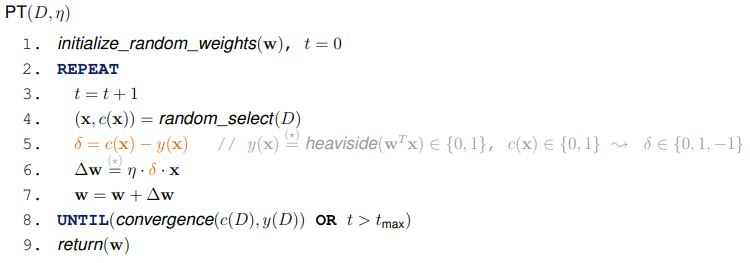
\includegraphics{PT}
\begin{itemize}
\item If a separating hyperplane between $X_0$ and $X_1$ exists, the PT algorithm will
converge. If no such hyperplane exists, convergence cannot be guaranteed.
\item A separating hyperplane can be found in polynomial time with linear
programming. The PT Algorithm, however, may require an exponential
number of iterations.
\item Classification problems with noise are problematic
\end{itemize}
\subsection{Gradient Descent}
\begin{itemize}
\item Finde den kürzesten Weg in ein Min/Max über partielle Ableitungen
\item The gradient of a function is the direction of steepest ascent or descent.
\end{itemize}
\subsubsection{Linear Regression + Squared Loss}

$$ L_2(\textbf{w}) = \dfrac{1}{2} \cdot \displaystyle\sum_{(\textbf{x}, c(\textbf{x})) \in D} (c(\textbf{x}) - y(\textbf{x}))^2$$

Jetzt müssen wir für jedes $w_i$ aus \textbf{w} eine partielle Ableitung machen um den weight vector zu updaten ($ \textbf{w} = \textbf{w} + \Delta \textbf{w}$)

$$ \Delta\textbf{w} =  \dfrac{ \delta }{\delta w_i} L_2 (\textbf{w}) = \eta \cdot \displaystyle\sum_D (c(\textbf{x}) - \textbf{w}^T\textbf{x}) \cdot \textbf{x}$$

$\eta$ = learning rate - a small positiv constant - legen wir selbst fest

\subsubsection{The Batch Gradient Descent (BGD) Algorithm}
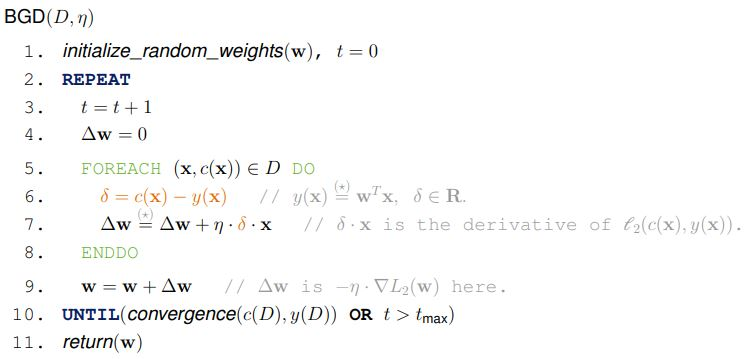
\includegraphics{BGD}
\begin{itemize}
\item wichtig: immer wenn irgendwo $\textbf{w}^T\textbf{x}$ steht haben wir $x_0 = 1$ zu \textbf{x} hinzugefügt
\item funktionsweise BGD. wir berechnen über die Ableitung in welche Richtung wir müssen und gehen dann einen Schritt der große $\eta$
\item die "convergence" schaut ob der Squared Loss noch größer als ein $\varepsilon$ ist (das wir auch festlegen)
\item BGD ist nicht der schnellste (aber sehr einfach) (Newton-Raphson algorithm, BFGS algorithm sind z.B. schneller)
\item BGD nimmt den global loss: loss of all examples in D (“batch gradient descent”)(Schritt in Richtung die für alle Punkte am besten ist)
\item man kann auch den (squared) loss in Bezug auf einzelne Beispiele nehmen (pointwise loss) (dann gehts halt im Zickzack runter)
\ berechnet sich dann $\ell_2(c(\textbf{x}), y(\textbf{x})) = \dfrac{1}{2} (c(\textbf{x})- \textbf{w}^T\textbf{x})^2$
\item bzw. die weight adaptation: $ \Delta\textbf{w} = \eta \cdot (c(\textbf{x}) - \textbf{w}^T \textbf{x}) \cdot \textbf{x} $
\item für $BGD_\sigma$ wird Zeile 9 zu  \\ $\textbf{w} = \textbf{w} + \Delta \textbf{w} + \eta \cdot 2 \lambda \cdot \binom{0}{\overrightarrow{\textbf{w}}}$
\end{itemize}
\subsubsection{The Incremental Gradient Descent IGD Algorithm}
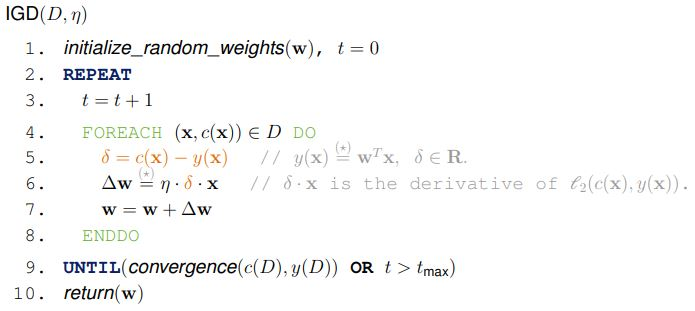
\includegraphics{IGD}
\begin{itemize}
\item kleinere Schritte als BGD
\item  can better avoid getting stuck in a local minimum of the loss function then BGD
\end{itemize}
\subsubsection{Logistic Regression + Logistic Loss + Regularization}
Wie oben nur mit neuer Formel für $\Delta \textbf{w}$:
$$ \Delta\textbf{w} = \eta \cdot \displaystyle\sum_D (c(\textbf{x}) - \sigma (\textbf{w}^T\textbf{x}))\cdot \textbf{x} - \eta \cdot 2 \lambda \cdot \binom{0}{\overrightarrow{\textbf{w}}} $$


\end{flushleft}
\end{document}
